\subsection{SPAD Matrices}

The binary response of the sensor defines the need for a subsequent signal amplification process to generate a sufficiently large voltage signal from a single photon. In one of the currently available gigapixel imaging technologies, this is achieved via the integration of the \textit{single-photon avalanche diode} (SPAD) structures, which implement gain mechanisms internally (\cite{Saleh1991}); this internal amplification process is referred to as electron \textit{avalanche multiplication}~\cite{Ma:17}. Since each detected photon is converted into a cascade of moving carrier pairs, even weak light can produce a clearly detectable current. %The depletion-layer electric field in a photodiode is increased by applying a sufficiently reverse bias across the junction so that the electrons and holes generated may acquire sufficient energy to liberate more electrons and holes within this layer by a process of impact ionization. \cite{Saleh1991} 

\begin{figure}[h]
  \centering
  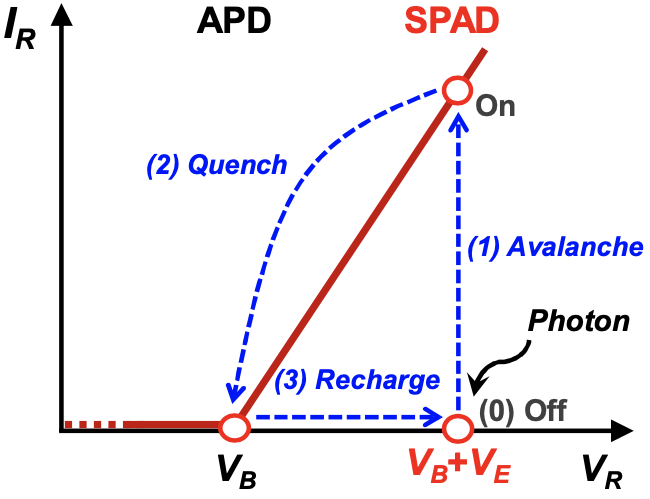
\includegraphics[width=0.8\linewidth]{imgs/spad/avalanche.png}
  \caption{SPAD operation process, demonstrating changes in voltage during the avalanche effect and subsequent quenching. Via \cite{Charbon2018}}
  \label{fig:avalanche}
  \Description{A diagram shows the shift in current during the SPAD-based acquisition process, which happens rapidly for a single photon. Later, the current must drop via quenching.}
\end{figure}

In avalanche photodiodes, the junction electric field is large enough such that the available carriers are accelerated, causing \textit{impact ionization}, i.e., producing further photoelectrons through collision. Ergo, high electrical voltage over 20V is required~\cite{Gnanasambandam_2019}; some prototypes, like the one described in \cite{rng16}, define even higher supply voltages of ca. 22–27V for biasing above breakdown. SPAD is operated in Geiger mode \cite{7117471}. For SPAD arrays, higher breakdown voltage is desirable in general, as it allows for higher photon detection efficiency and improved timing resolution~\cite{7117471}.

The first proposal for a fully integrated CMOS SPAD array has been reported in \cite{Rochas2003}. \cite{DuttonSPAD} allude to other SPAD detectors which have been developed since, noting the variety in both general form (single-point detectors, line sensors, large array photomultipliers, and image sensors) and pixel designs; subsequently, it is stated that no single SPAD-based pixel architecture has been deemed dominant to date. 

The fast detection times in SPADs are associated with the rapidity of the impact ionization process. However, each photon detection event must be followed by finite recovery time, in which the diode is restored to the operative level voltage-wise, freeing excess charge carriers. This process is called \textit{quenching}. During this time, device does not respond to further incident photons. To enable quenching, additional in-pixel circuitry is needed.
Due top the larger amount of transistors needed per single photodetector, the fill-factor of SPAD-based pixels is limited (<40\%), and so is the quantum efficiency (<30\%)~\cite{Ma:17}.

Generally, the SPAD devices aren't entirely compatible with the CMOS technologies due to high operating voltage requirements; the necessity for a large electric field and additional readout circuitry results in the larger dimensions of the structure, lower spatial resolution and higher power dissipation~\cite{Ma:17}. Furthermore, the generation of electrons is based on thermal reactions, rendering the detectors significantly more susceptible to dark current.

However, significant progress has been achieved in recent years~\cite{SPADperformance, rng16}. Performance of SPAD-based architecture using the developments in 3D stacking technologies is described in detail in \cite{Charbon2018}.


